\documentclass{article}
\usepackage[a4paper,top=3cm,bottom=2cm,left=3cm,right=2cm]{geometry}
\usepackage[utf8]{inputenc}
\usepackage[T1]{fontenc}
\usepackage{graphicx}

\title{Rapport Technique d'évaluation}
\date{20 Juillet 2021}

\begin{document}
\maketitle

\begin{figure}[!t] 
    \center 
    
\includegraphics{banniere.png} 
\end{figure}

	\section*{Présentation}

	\begin{itemize}	
	
		\item \textbf{Projet :} Analyse de radiographies pulmonaires Covid-19
	
		\item \textbf{Promotion :} DS Octobre 2020
				
		\item \textbf{Membres de l'équipe}
			
		\begin{itemize}
			\item Potrel Manuel
			\item Amuli Inès
			\item Ngoma Algy
			\item Turlet Frédéric
		\end{itemize}
		
		\item \textbf{Mentor :} Paul Dechorgnat
		
	\end{itemize}
	
	\newpage	
	\section*{Contexte}
	
	~ 
	\par Face à la situation sanitaire actuelle, des solutions et alternatives pour la détection du Covid-19 sont très recherchées. L'analyse de radiographies pulmonaires est une possibilité à explorer, les modèles de Deep Learning s'étant déjà montrés extrêmement performants dans le domaine de l'imagerie médicale.
	\par Si la classification se révèle efficace pour détecter les cas positifs, alors cette méthode peut être utilisée dans les hôpitaux et cliniques comme alternative aux tests classiques.
	\par Cependant, il reste toujours à prouver qu'il est possible de détecter le virus uniquement à l'aide de radiographies de poumons.
	
	\section*{Data}
	
	~
	\par Le jeu de données fut téléchargé depuis le site Kaggle.\\
	Il s'agit d'images de radiographies pulmonaires de patients appartenant à l'une des trois catégories suivantes :
	
	\begin{enumerate}
	
		\item COVID-19 : 1141 images de dimensions variées
		\item NORMAL : 1343 images de dimension $1024 \times 1024$
		\item Viral Pneumonia : 1345 images de dimension $1024 \times 1024$
		
	\end{enumerate}
	
	\par Ce jeu de données occupe un poids d'environ 1.15 Go.\\
	Voici quelques exemples d'images sélectionnées aléatoirement.
	
	\begin{figure}[!h] 
    \center 
    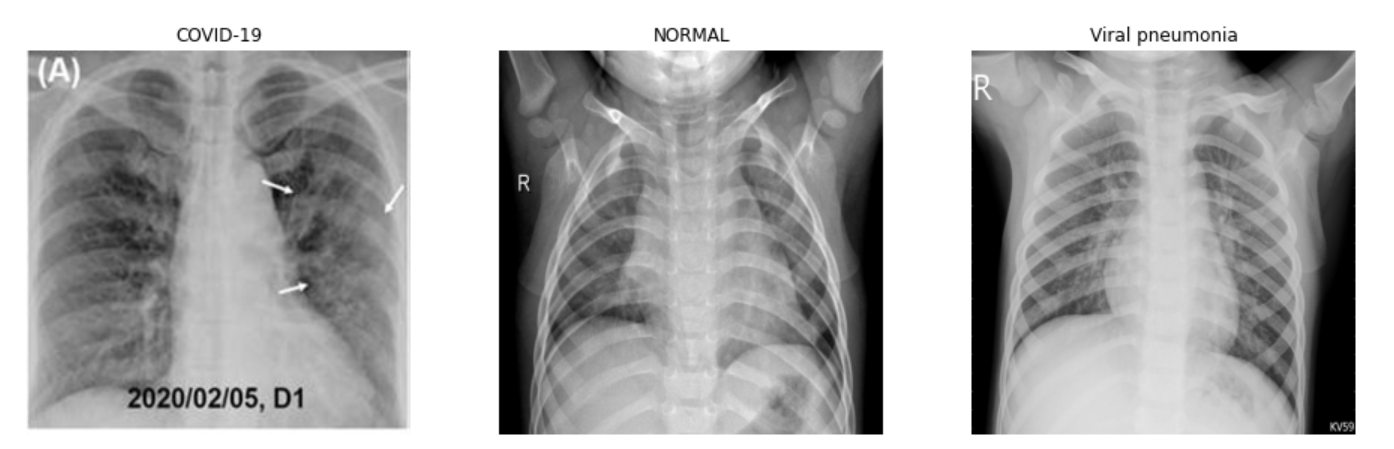
\includegraphics[scale=0.3]{exemples_img.png} 
	\end{figure}
	
	\par Plusieurs challenges ont été rencontrés au cours du projet. La nature et la complexité de ces problèmes étaient très variées.
	
	\par Il est apparent que les images des classes NORMAL et Viral Pneumonia sont d'un standard très différent de celui des images de la classe COVID-19.
	\par Une importante quantité de ces dernières contient différents éléments externes aux poumons du patient. On peut observer des tubes de différentes tailles, des annotations fléchées ou même des écritures.
	
	\par Par ailleurs, alors que la position des patients semble être la même pour les deux autres classes, on trouve des patients positionnés en biais, ou plus haut (ou plus bas) dans les données COVID-19. Beaucoup d'entre eux ne lèvent pas non plus les bras.
	
	\par Une autre différence importante est que, pour beaucoup de patients infectés par le covid, il semble que l'image soit déjà zoomée sur les poumons.\\
	Afin de remédier à ce problème, il a fallu construire une fonction permettant de zoomer sur les poumons lorsque l'intensité des pixels au bord de l'image était inférieure à un certain seuil dépendant de l'intensité moyenne de l'image.
	
	\par Enfin, il semble que même les patients soient de constitution différente, comme on peut le voir par la forme des poumons sur le graphique ci-dessous, représentant une moyenne des images pour chaque classe.
	
    \begin{center}
         
    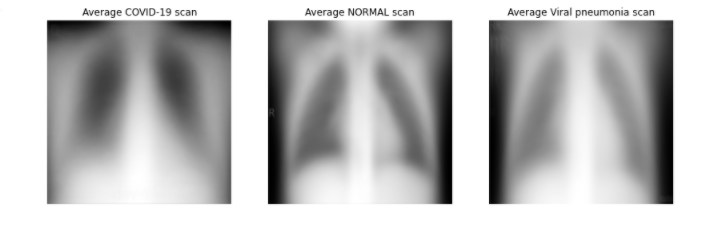
\includegraphics[scale=0.5]{avg_img.png} 
    
	\end{center}
    
    \par La dernière variation sur les données ne provient, cette fois-ci, pas du contenu des images mais de leur dimension.\\
    Les images des patients COVID-19 ne sont pas systématiquement d'une résolution de $1024 \times 1024$, c'est même plutôt rare.\\
    Il a donc fallu faire un choix entre redimensionner toutes les images COVID-19 en $1024 \times 1024$ ou choisir une taille moins élevée. La seconde méthode a l'avantage de réduire le poids du dataset et de ne pas modifier trop drastiquement certaines images COVID-19. Le choix d'une dimension de $256 \times 256$ a ensuite été pris.
	
	\section*{Projet}
	
	\subsubsection*{Exploration}
	
	\par Lors de l'exploration des données, nous cherchions à mettre en évidence des indicateurs potentiels permettant de différencier les classes.
	
	\par Nous avons utilisé des techniques de visualisation à l'aide des libraries \textit{matplotlib} et \textit{seaborn} pour trouver des pistes à approfondir.
	
	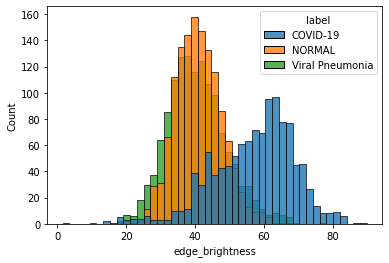
\includegraphics[scale=0.6]{edge_intensity.png}
	
	\par On voit ci-dessus un histogramme qui semble révéler que l'intensité des pixels sur les bords verticaux de l'image pourrait être un indicateur permettant de repérer les images classées COVID-19.\\
	Ci-dessous, on trouve un autre histogramme permettant à nouveau d'exposer cette classe, cette fois-ci en étudiant le nombre de pixels d'intensité inférieure à 50.
	
	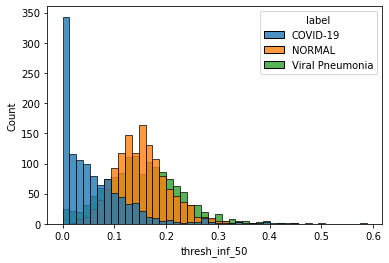
\includegraphics[scale=0.6]{intensity_thresh.png}
		
	\par Après avoir identifié une certaine quantité d'indicateurs, nous avons utilisé un test statistique : le test ANOVA de la librairie \textit{statsmodels}.\\
	Dans un contexte où nous voulons étudier la relation entre une variable qualitative et une variable quantitative, ce test permet de rejeter, ou non, l'hypothèse que la moyenne de la variable quantitative est indépendante de la variable qualitative.\\
	Dans notre cas, pour tous les indicateurs étudiés, le test a révélé que les moyennes variaient selon la classe. Autrement dit, il y a une corrélation entre appartenir à une certaine classe et posséder une certaine intensité moyenne de pixels.
	
	\subsubsection*{Gestion des biais}
	
	\par Afin de combattre les biais, il a fallu développer plusieurs fonctions de preprocessing.\\
	Voici celui que nous avons choisi (un zoom accompagné d'un traitement d'intensité).
	\begin{center}
	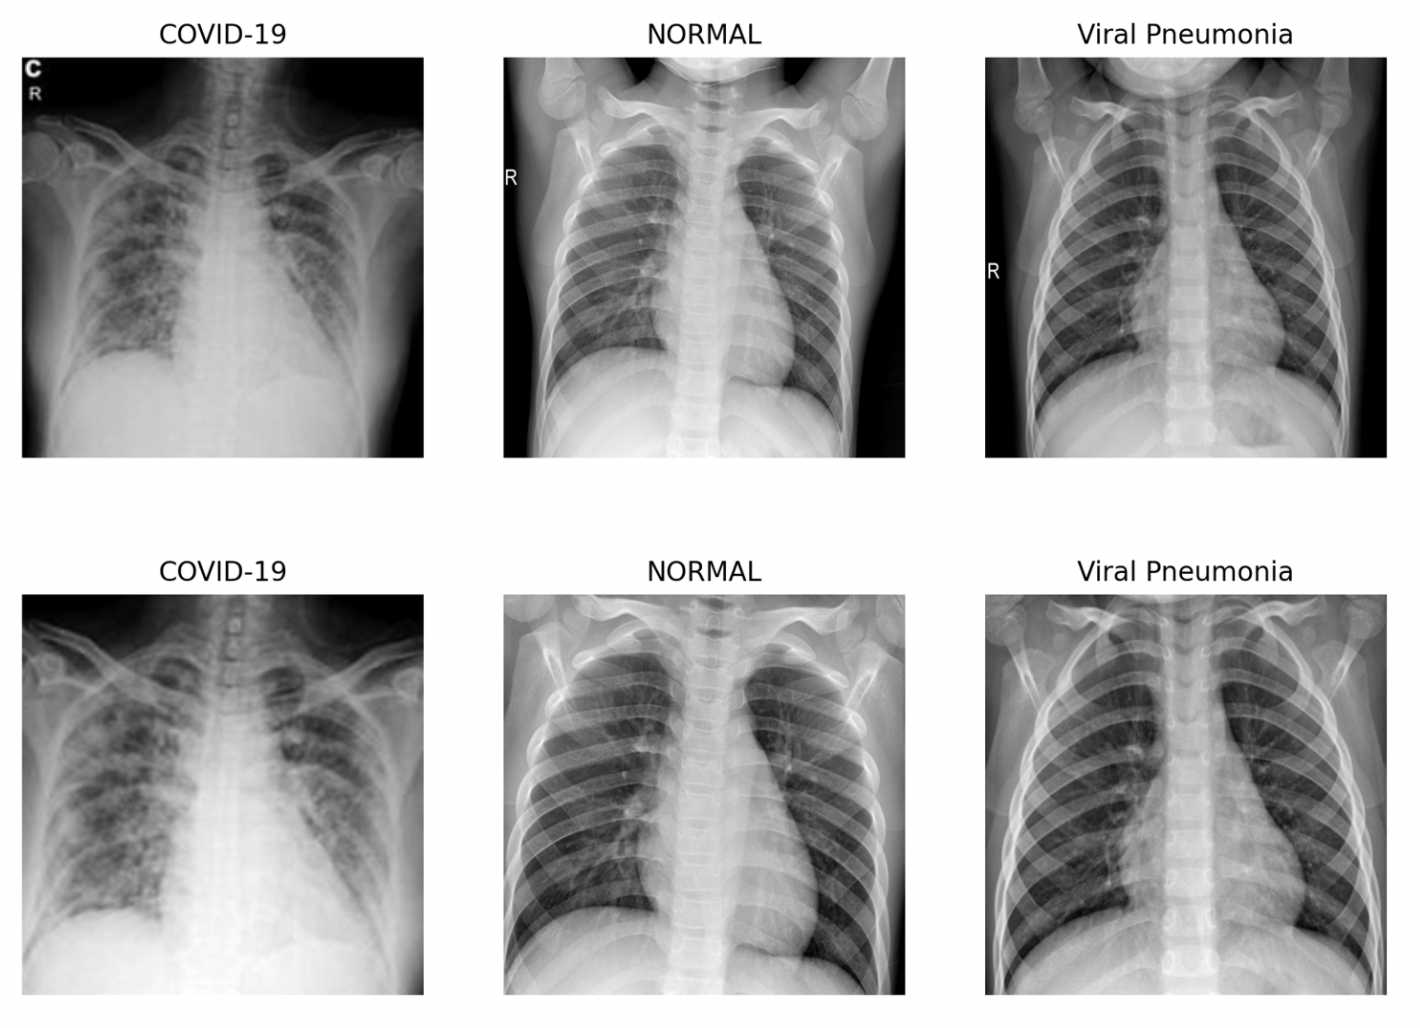
\includegraphics[scale=0.4]{preprocess.png}
	\end{center}	
	
	\par En plus de la librairie \textit{numpy}, utilisée pour manipuler la forme matricielle des images, nous avons utilisé des librairies de traitement d'image, comme \textit{OpenCV}, \textit{PIL} et \textit{Scikit-image} afin de jouer sur l'intensité et le contraste (parmi d'autres critères).
	
	\par Pour chaque preprocessing, il a fallu également trouver une façon d'évaluer la quantité de biais restants. Pour cela, nous avons utilisé deux techniques de réduction de dimensionnalité.
	
	\begin{center}
	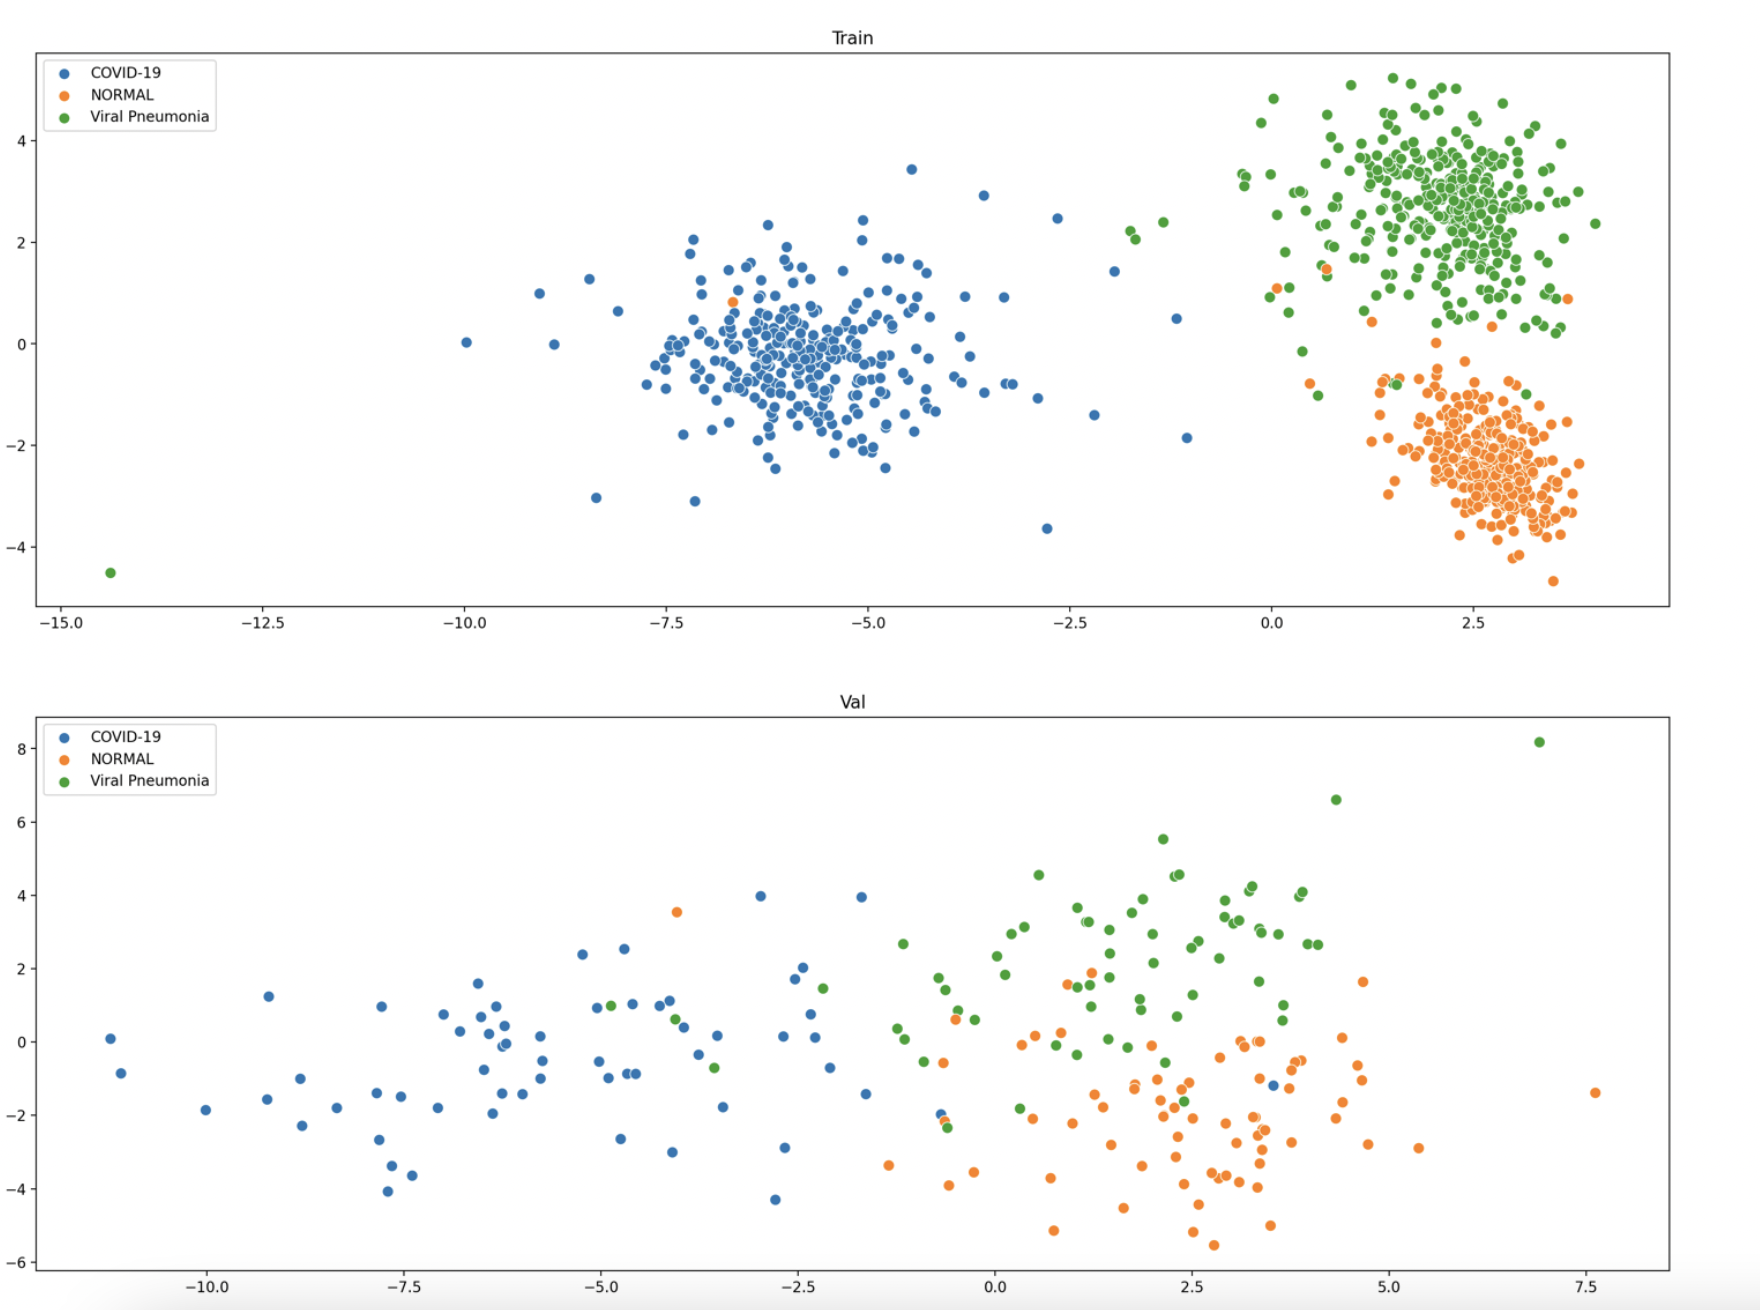
\includegraphics[scale=0.4]{lda.png}
	\end{center}	
	
	\par Sur l'image ci-dessus, vous pouvez observer le résultat d'une technique appelée LDA, permettant de réduire la dimension d'un vecteur de features, en prenant en compte son label de classification. Nous répétons ensuite les projections (graphique du bas) sur un ensemble de test pour voir si les clusters se positionnent toujours de la même façon, relativement aux autres classes. Nous avons utilisé la librairie \textit{sklearn} pour cet algorithme.\\
	Nous appliquons ensuite une technique d'ensemble en Machine Learning, un classifieur Random Forest (toujours de la librairies \textit{sklearn}), entraîné sur le jeu transformé par la LDA et évalué sur le jeu de test.\\
	L'idée de cette technique est que si de simples manipulations linéaires suffisent pour qu'un classifieur qui n'est pas un réseau de neurone parvienne à identifier les trois classes relativement correctement, c'est qu'il reste une quantité de biais suffisamment importante.
	
	\par Une autre technique de réduction de dimensionnalité, ici du Manifold Learning, n'utilisant pas les labels mais permettant de simplifier l'étude des données de façon non linéaire, est appelée t-SNE.\\
	Similairement à la LDA, la présence de clusters est un signe que les données gardent encore des biais.
	
	\begin{center}
	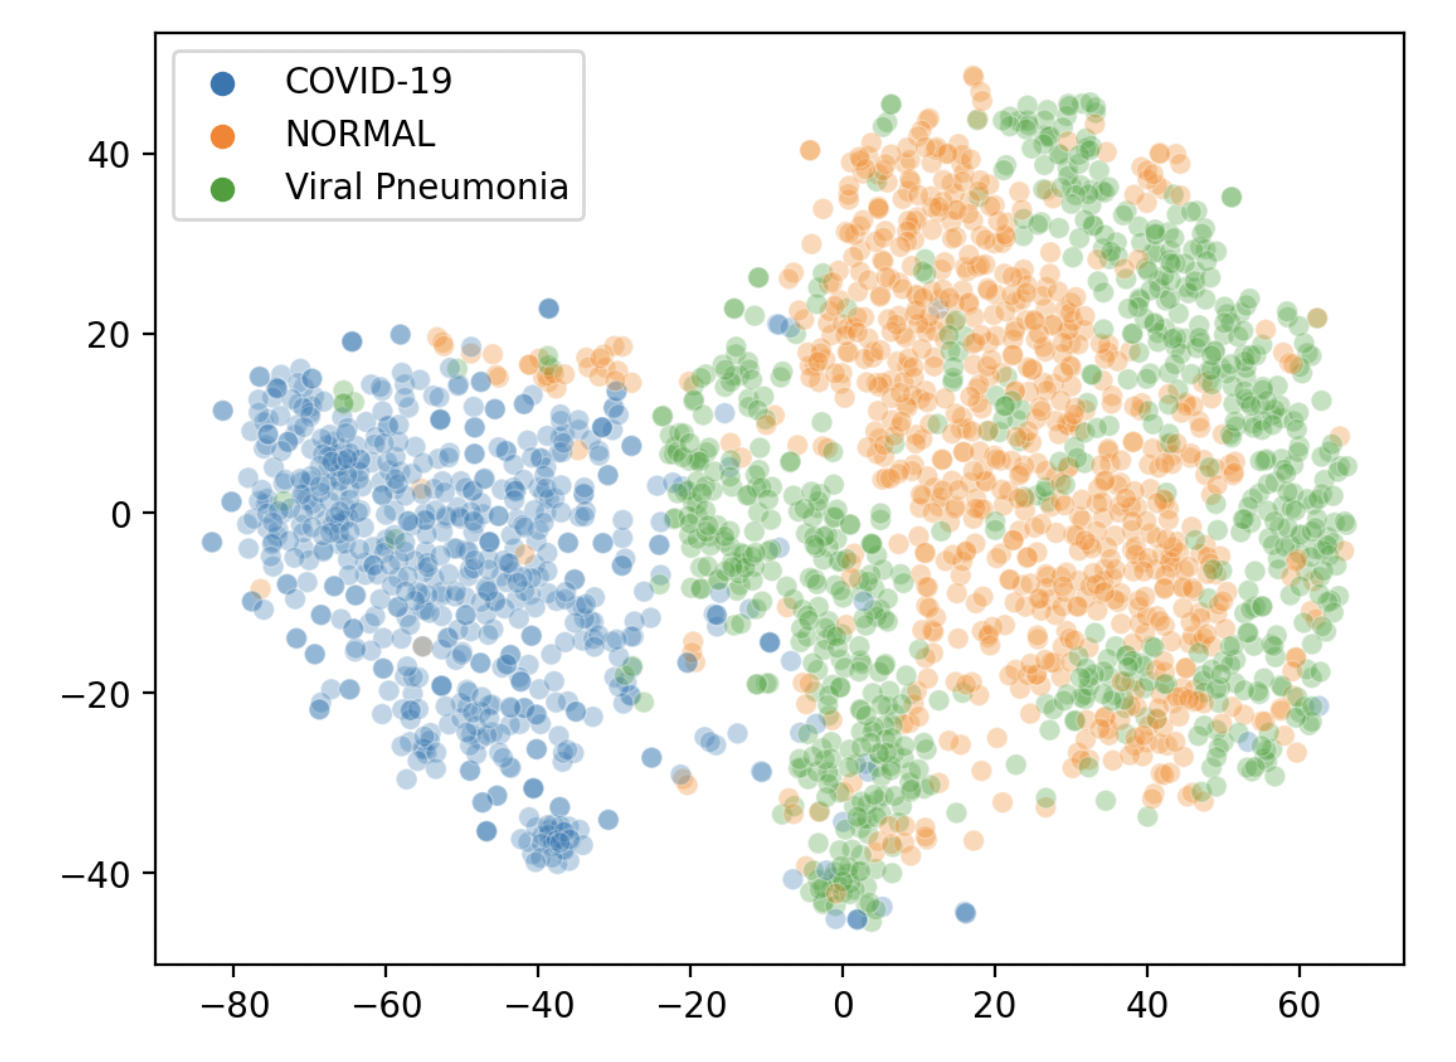
\includegraphics[scale=0.5]{tsne.png}
	\end{center}
	
	Aucun des preprocessings testés n'a permis de réduire les biais de façon satisfaisante, tous les classifieurs obtenaient une précision de plus de 80\%.\\
	Il a donc fallu imaginer une technique de visualisation pour comparer les preprocessings et en choisir un (dans notre cas, un zoom accompagné d'un traitement d'intensité).\\
	La technique choisie ici est l'application de boxplots permettant, pour chaque preprocessing en abscisse, de comparer la distribution des valeurs d'un indicateur.
	
	\begin{center}
	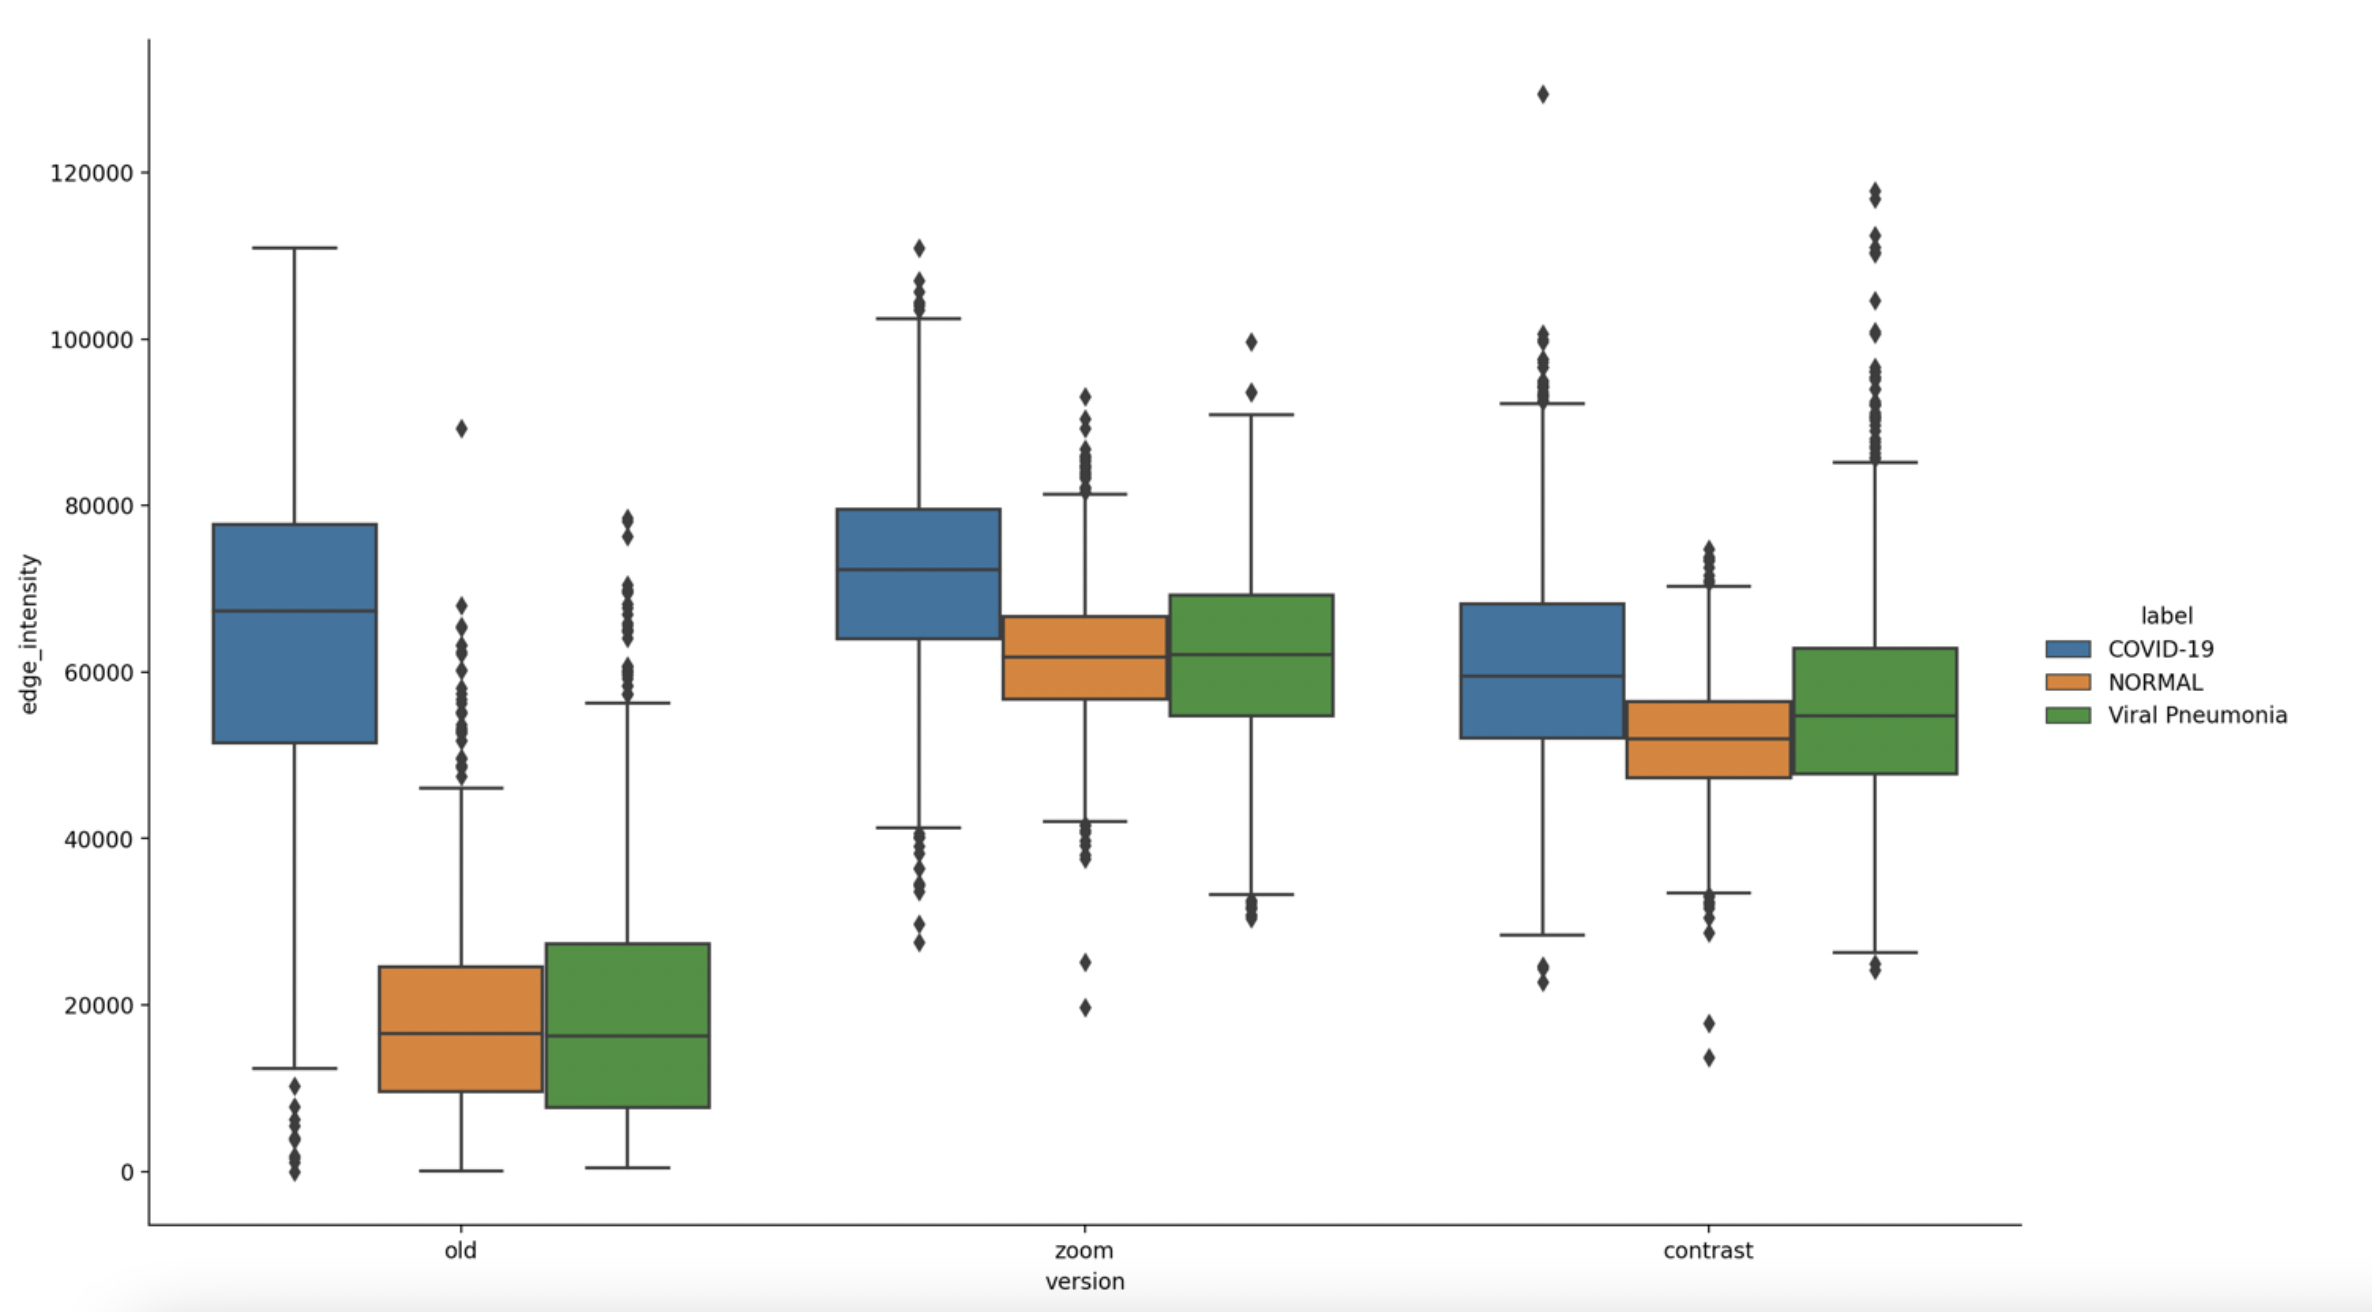
\includegraphics[scale=0.3]{preprocess_comp.png}
	\end{center}
	
	Enfin, la dernière tentative que nous avons faite est celle liée au réseau de neurones \textbf{U-Net}. Construit grâce à \textit{TensorFlow}, ce réseau de neurones convolutionnel permet de segmenter les images, c'est à dire d'isoler certaines parties qui nous intéressent. Dans notre cas, il s'agit des poumons.
	
	\begin{center}
	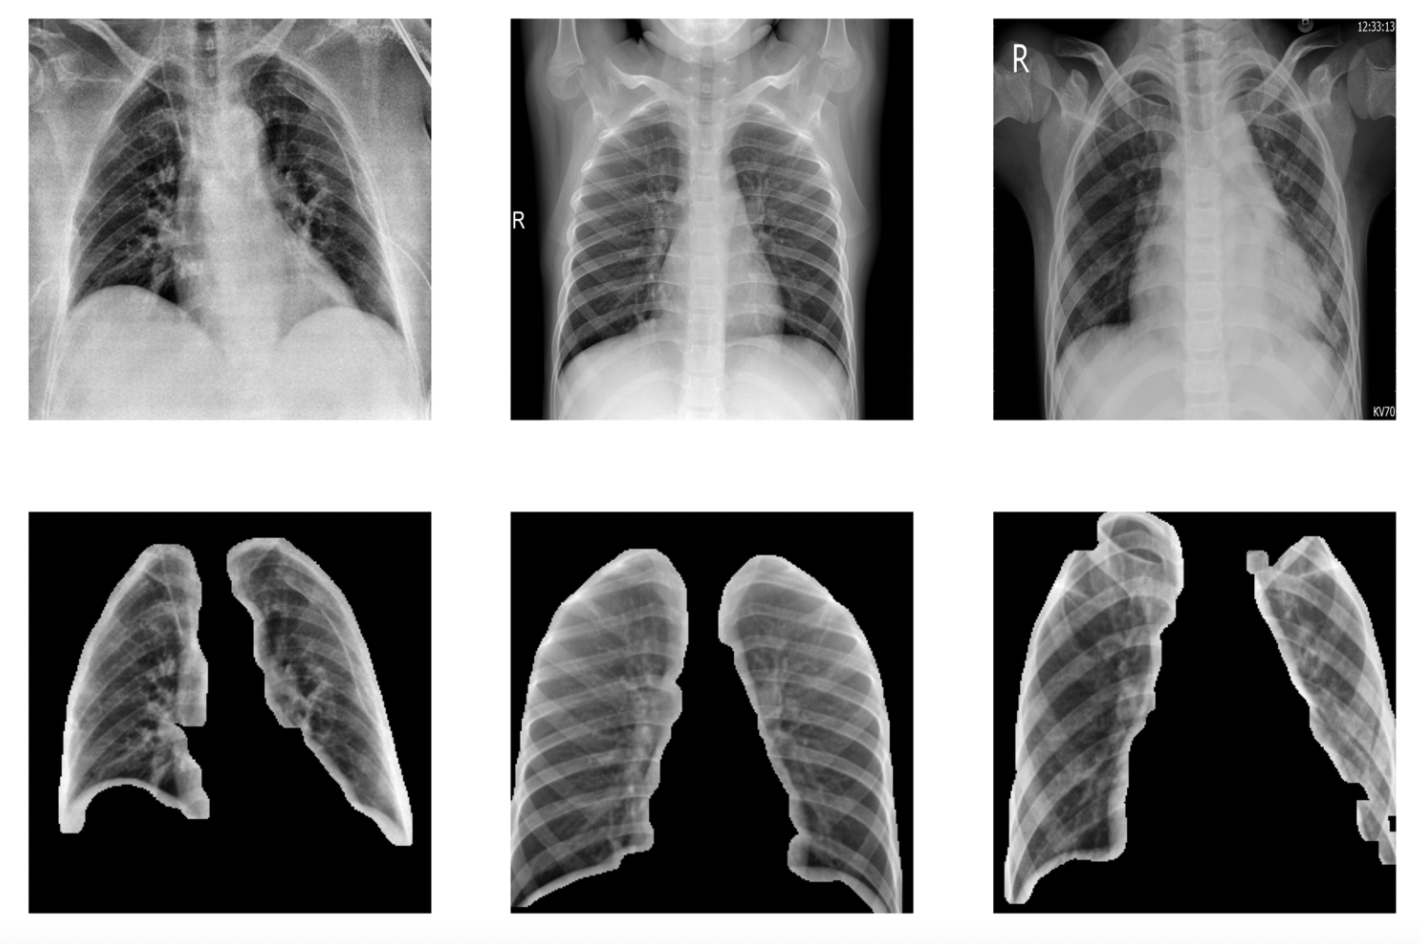
\includegraphics[scale=0.6]{unet.png}
	\end{center}
	
	\subsubsection*{Classification}

	Pour la classification, nous avons testé diverses architectures de réseaux de neurones convolutionnels grâce à la librairie \textit{TensorFlow}.\\
	Nous avons retenu deux architectures principales. L'une d'entre elle fut construite grâce à la classe \textit{Sequential}, permettant d'empiler les couches de neurones, et contient deux blocs de convolution et deux couches denses.\\
	Pour le second, nous avons répliqué l'architecture \textbf{VGG-16}, une architecture bien plus compliquée qui s'est démarquée dans la classification d'images.
	
	\begin{center}
	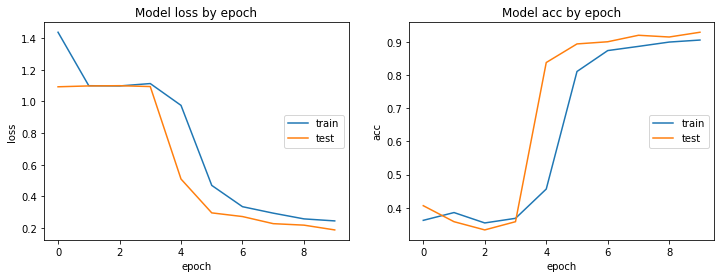
\includegraphics[scale=0.5]{acc_vgg_zb.png}
	\end{center}
	
	\subsubsection*{Interprétabilité}
	
	Une fois que les réseaux de neurones étaient entraînés, nous avons décidé d'étudier leurs méthodes de classification et de comprendre leurs critères.\\
	Pour cela, nous avons sélectionné la technique nommée \textbf{Grad-CAM}, permettant de créer une heatmap à calquer sur l'image originale afin de mettre en évidence les pixels qui ont joué les plus grands rôles dans la décision.
	
	\begin{center}
	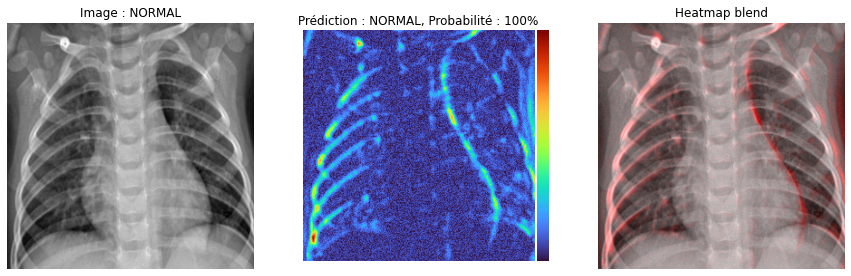
\includegraphics[scale=0.5]{interp.png}
	\end{center}
	
	\subsubsection*{Déploiement}
	
	Enfin, pour le déploiement de notre application sur le web, nous avons utilisé l'API \textbf{Streamlit}, permettant de présenter notre projet ainsi que d'effectuer une prédiction par notre modèle de toute image fournie par le client visiteur.
	
	\section*{Difficultés}
	
	La difficulté principale que nous avons rencontrée dans ce projet est celle de la gestion des biais. Nous n'avons pas trouvé de façon de contrer ce problème et il a donc fallu prendre des décisions, par exemple le choix des modèles, en sachant que de bonnes prédictions n'étaient pas forcément synonyme de bon modèle.\\
	Bien évidemment, le fait de ne pas réussir à atténuer les biais représente en lui-même une grande difficulté.
	
	\par Un autre obstacle auquel il a fallu faire face est celui de l'inconnu. Nous avons dû découvrir de nouvelles librairies, notamment pour le traitement d'image et le déploiement, mais également de nouvelles techniques.\\
	Il a également été nécessaire de comprendre, dans une certaine mesure, leur fonctionnement théorique afin de pouvoir nous débloquer quand nous faisions face à des bugs où à des résultats que nous ne nous expliquions pas.\\
	Ce qui nous a fait défaut ici, c'est l'expérience et la pratique.
	
	\'Etant un groupe de quatre, nous avons eu plusieurs désaccords sur la façon de gérer le projet, sur la pertinence de certaines parties mais également simplement sur la façon de lire les données. Ces problèmes, qui furent largement résolus lors de la première moitié du projet, auraient pu être évités en communiquant plus fréquemment entre nous, notamment en utilisant dès le début la plateforme \textbf{GitHub}.
	
	\section*{Bilan}

	Les résultats de nos réseaux de neurones sur le jeu de données (entraînement et validation) sont excellents en théorie. Néanmoins, quand on l'essaye sur un jeu externe, il se trouve que les prédictions deviennent médiocre.\\
	Le projet n'est donc pas actuellement utilisable, en tout cas pas avec un certain seuil d'exigence, mais il forme un début de recherche dans ce domaine.\\
	Nous avons trouvé trois conclusions possibles.
	
	\begin{enumerate}

		\item Il n'est pas possible de déterminer si un patient est atteint du covid à partir d'une radiographie de ses poumons.
		\item Notre jeu de données était trop biaisé pour qu'un modèle puisse repérer les patternes réellement importants, quel que soient les preprocessings appliqués en amont.
		\item Un preprocessing permettant d'aider un modèle à réellement repérer les patternes importants sur des poumons pour cette classification précise existe, mais nous ne l'avons pas trouvé.
	
	\end{enumerate}
	
	Le temps (et probablement les prochaines compétitions sur Kaggle) nous apportera plus d'informations sur ces hypothèses.
	
	Dans tous les cas, ce projet nous a permis à tous de gagner en confiance et en expérience avec le langage Python, d'apprendre à rechercher solutions aux problèmes, de travailler en équipe et de découvrir les différentes étapes (et bonnes pratiques) d'un projet de Data Science.  

\end{document}